\documentclass[]{book}
\usepackage{lmodern}
\usepackage{amssymb,amsmath}
\usepackage{ifxetex,ifluatex}
\usepackage{fixltx2e} % provides \textsubscript
\ifnum 0\ifxetex 1\fi\ifluatex 1\fi=0 % if pdftex
  \usepackage[T1]{fontenc}
  \usepackage[utf8]{inputenc}
\else % if luatex or xelatex
  \ifxetex
    \usepackage{mathspec}
  \else
    \usepackage{fontspec}
  \fi
  \defaultfontfeatures{Ligatures=TeX,Scale=MatchLowercase}
\fi
% use upquote if available, for straight quotes in verbatim environments
\IfFileExists{upquote.sty}{\usepackage{upquote}}{}
% use microtype if available
\IfFileExists{microtype.sty}{%
\usepackage{microtype}
\UseMicrotypeSet[protrusion]{basicmath} % disable protrusion for tt fonts
}{}
\usepackage[margin=1in]{geometry}
\usepackage{hyperref}
\hypersetup{unicode=true,
            pdftitle={SOC 4650/5650 User's Guide},
            pdfauthor={Christopher Prener, Ph.D.},
            pdfborder={0 0 0},
            breaklinks=true}
\urlstyle{same}  % don't use monospace font for urls
\usepackage{natbib}
\bibliographystyle{apalike}
\usepackage{longtable,booktabs}
\usepackage{graphicx,grffile}
\makeatletter
\def\maxwidth{\ifdim\Gin@nat@width>\linewidth\linewidth\else\Gin@nat@width\fi}
\def\maxheight{\ifdim\Gin@nat@height>\textheight\textheight\else\Gin@nat@height\fi}
\makeatother
% Scale images if necessary, so that they will not overflow the page
% margins by default, and it is still possible to overwrite the defaults
% using explicit options in \includegraphics[width, height, ...]{}
\setkeys{Gin}{width=\maxwidth,height=\maxheight,keepaspectratio}
\IfFileExists{parskip.sty}{%
\usepackage{parskip}
}{% else
\setlength{\parindent}{0pt}
\setlength{\parskip}{6pt plus 2pt minus 1pt}
}
\setlength{\emergencystretch}{3em}  % prevent overfull lines
\providecommand{\tightlist}{%
  \setlength{\itemsep}{0pt}\setlength{\parskip}{0pt}}
\setcounter{secnumdepth}{5}
% Redefines (sub)paragraphs to behave more like sections
\ifx\paragraph\undefined\else
\let\oldparagraph\paragraph
\renewcommand{\paragraph}[1]{\oldparagraph{#1}\mbox{}}
\fi
\ifx\subparagraph\undefined\else
\let\oldsubparagraph\subparagraph
\renewcommand{\subparagraph}[1]{\oldsubparagraph{#1}\mbox{}}
\fi

%%% Use protect on footnotes to avoid problems with footnotes in titles
\let\rmarkdownfootnote\footnote%
\def\footnote{\protect\rmarkdownfootnote}

%%% Change title format to be more compact
\usepackage{titling}

% Create subtitle command for use in maketitle
\newcommand{\subtitle}[1]{
  \posttitle{
    \begin{center}\large#1\end{center}
    }
}

\setlength{\droptitle}{-2em}
  \title{SOC 4650/5650 User's Guide}
  \pretitle{\vspace{\droptitle}\centering\huge}
  \posttitle{\par}
  \author{Christopher Prener, Ph.D.}
  \preauthor{\centering\large\emph}
  \postauthor{\par}
  \predate{\centering\large\emph}
  \postdate{\par}
  \date{2017-01-28}

\usepackage{booktabs}

\begin{document}
\maketitle

{
\setcounter{tocdepth}{1}
\tableofcontents
}
\chapter*{Preface}\label{preface}
\addcontentsline{toc}{chapter}{Preface}

This text is a companion document for \textbf{SOC 4650/5650 -
Introduction to Geographic Information Sciences}. It is designed to help
you be \emph{successful} in this course. The idea behind a course
\textbf{User's Guide} is to create a reference for many of the
intangible, subtle or disparate skills and ideas that contribute to
being a successful researcher. In creating a \textbf{User's Guide}, I
draw inspiration from the work of Donald Knuth.\footnote{\href{https://en.wikipedia.org/wiki/Donald_Knuth}{Donald
  Knuth} is the developer of
  \href{https://en.wikipedia.org/wiki/TeX}{TeX}, a computer typesetting
  system that is widely used today for scientific publishing in the form
  of \href{https://en.wikipedia.org/wiki/LaTeX}{LaTeX}. He also
  established the concept of
  \href{https://en.wikipedia.org/wiki/Literate_programming}{literatue
  programming}, which forms the basis of some of the practices we will
  follow with Stata this semester.} Knuth has discussed his experiences
in designing new software languages, nothing that the developer of a new
language

\begin{quote}
\ldots{}must not only be the implementer and the first large-scale user;
the designer should also write the first user manual\ldots{} If I had
not participated fully in all these activities, literally hundreds of
improvements would never have been made, because I would never have
thought of them or perceived why they were important\ldots{}
\end{quote}

While there is nothing particularly new about what I am writing here,
and I am certainly not developing a new language for computing, the goal
of the \textbf{User's Guide} remains similar to Knuth's experience. By
distilling some of key elements for making a successful transition to
being a \emph{professional developer} of knowledge rather than a
\emph{casual consumer}, I hope to both improve the course experience
itself and also create an environment that fosters a successful learning
experience for you.

If you read through the course objectives included in the syllabus, you
will note that creating maps is only one of them. As much as this is a
GIS course, it is a course in research methods. In particular, we are
concerned with \emph{high quality} research methods and the
\emph{process} of conducting research. We therefore focus on a
combination of mental habits and technical practices that make you a
successful researcher. Some of the skills and techniques that we will
discuss this semester are not taught as often in graduate programs.
Instead, they are often the products of ``learning the hard way''. These
``habits of mind and habits of method'' are broadly applicable across
methodologies and disciplines.

\section*{License}\label{license}
\addcontentsline{toc}{section}{License}

Copyright © 2016-2017 \href{http://chrisprener.net}{Christopher G.
Prener}

This work is licensed under a Creative Commons Attribution 4.0
International License.

\chapter{Getting Started}\label{gettingStarted}

Before you begin the semester, there are a number of things that I
recommend that you do to help set yourself up for success. Before you do
\emph{anything} else, you should read through the
\href{}{\textbf{Syllabus}} and the \href{}{\textbf{Reading List}}. Make
sure you have a good sense of what is \emph{required} for the course. If
you have questions, bring them to the first day of class!

\section{Prep Your Computer}\label{prep-your-computer}

Before you do anything else for this course, make sure you get your
computer ready for the work you are about to undertake:

\begin{enumerate}
\def\labelenumi{\arabic{enumi}.}
\tightlist
\item
  Make sure your operating system is up-to-date. If you are able, I
  would also recommend upgrading your computer to the most recent
  release of its operating system that the computer can run.
\item
  We'll be sharing computer files throughout the semester, so you should
  ensure that you have functioning anti-virus software and that it is
  up-to-date.
\item
  You'll also need to download files, so you'll need to make sure you
  have some free space on your hard drive. If you have less than 10GB of
  free space, you should de-clutter!
\item
  Make sure you know how to access your computer's file management
  system.

  \begin{itemize}
  \tightlist
  \item
    On macOS, this means being comfortable with Finder.app.
  \item
    On Windows, this means being comfortable with Windows Explorer.
  \end{itemize}
\end{enumerate}

This of course assumes that you own a computer. Owning a computer is not
required for this course. All students who are enrolled in SOC 4650 or
SOC 5650 will be given 24-hour swipe access (\emph{just what you always
wanted!}) to Morrissey Hall to facilitate access to lab computers.

\section{Create Accounts}\label{create-accounts}

There are two major web services that we will use this semester, and
you'll need to create accounts for both:

\begin{itemize}
\tightlist
\item
  \textbf{GitHub} - you can sign-up at
  \href{https://github.com}{GitHub.com}. Once you've signed up, fill out
  your profile, set-up
  \href{https://help.github.com/articles/about-two-factor-authentication/}{two-factor
  authentication}, and let Chris know (via
  \href{mailto:prenercg@slu.edu}{email}) what your user name is. Once he
  has it, he can add you to the
  \href{https://github.com/slu-soc5650}{SOC 4650/5650} organization.
\item
  \textbf{Slack} - you can ask Chris (via
  \href{mailto:prenercg@slu.edu}{email}) for an invitation to sign-up
  for our team. Once the sign-up process is complete, you can log-in by
  going to our team's \href{https://slu-soc5650.slack.com}{Slack site}.
  Fill out your profile, set-up
  \href{https://get.slack.help/hc/en-us/articles/204509068-Set-up-two-factor-authentication}{two-factor
  authentication}, and change your timezone.
\end{itemize}

\section{Download and Install
Software}\label{download-and-install-software}

There are a number of software applications that we will use this
semester. Most of them are free, and I recommend downloading those free
ones right away. All of these applications are available for macOS and
Windows.

\begin{itemize}
\tightlist
\item
  \textbf{Atom} - Atom is a flexible, open-source text editor that is
  produced by GitHub. You can download it from Atom's
  \href{https://atom.io}{website}.
\item
  \textbf{GitHub Desktop} - GitHub makes a desktop client that you can
  use to easily interact with repositories that are stored on the site.
  You can download it from GitHub's
  \href{https://desktop.github.com}{website} after you sign-up for an
  account there. You'll need that account information to complete the
  desktop client's set-up process.
\item
  \textbf{Slack} - Slack has a number of applications for desktop and
  mobile operating systems. I recommend downloading Slack on your
  personal computer, and optionally installing it on your mobile device
  as well. You can download their desktop applications from their
  \href{https://slack.com/downloads}{website} and the mobile
  applications from your App Store.
\end{itemize}

\subsection*{\texorpdfstring{For Graduate Students
\emph{only}}{For Graduate Students only}}\label{for-graduate-students-only}
\addcontentsline{toc}{subsection}{For Graduate Students \emph{only}}

If your computer meets the
\href{http://desktop.arcgis.com/en/arcmap/10.3/get-started/system-requirements/arcgis-desktop-system-requirements.htm}{operating
system requirements} for ArcGIS and you think you'd benefit from having
access to the software at home, let Chris know (via
\href{mailto:prenercg@slu.edu}{email}).

If you are in the Public and Social Policy Ph.D.~program and your
computer meets the
\href{http://www.stata.com/support/faqs/windows/hardware-requirements/}{hardware}
and
\href{http://www.stata.com/products/compatible-operating-systems/}{software}
requirements for Stata, you should consider
\href{https://www.stata.com/order/new/edu/gradplans/student-pricing/}{purchasing
it} for yourself. I recommend purchasing a perpetual license for
Stata/IC. This is the most cost-effective solution for typical students.

\section{Buy Course Materials}\label{buy-course-materials}

\subsection*{Books}\label{books}
\addcontentsline{toc}{subsection}{Books}

There are three required books for this course:

\begin{enumerate}
\def\labelenumi{\arabic{enumi}.}
\tightlist
\item
  Brewer, Cynthia. 2015. \emph{Designing Better Maps: A Guide for GIS
  Users}. Redlands, CA: ESRI Press. ISBN-13: 978-1589484405; List Price:
  \$59.99; ebook versions available.
\item
  Gorr, Wilpen L. and Kristen S. Kurland. 2013. \emph{GIS Tutorial 1:
  Basic Workbook}. 10.3.x edition. Redlands, CA: ESRI Press. ISBN-13:
  978-1589484566; List Price: \$79.99; ebook versions available.
\item
  Thomas, Christopher and Nancy Humenik-Sappington. 2009. \emph{GIS for
  Decision Support and Public Policy Making}. Redlands, CA: ESRI Press.
  ISBN-13: 978-1589482319; List Price: \$24.95.
\end{enumerate}

There is one additional book that is optional:

\begin{itemize}
\tightlist
\item
  Mitchell, Michael N. 2010. \emph{Data Management Using Stata: A
  Practical Handbook}. College Station, TX: Stata Press. ISBN-13:
  978-1597180764; List Price: \$48.00.
\end{itemize}

Buying Mitchell (2010) is \emph{highly} recommended for graduate
students who will continue using Stata in the future and those who are
concerned about the command-line interface. I recommend waiting for a
week or two before purchasing this.

\subsection*{External Media}\label{external-media}
\addcontentsline{toc}{subsection}{External Media}

You will need a USB external storage device (either an external hard
drive or a thumb-style drive) that has at least 20GB of storage
capacity. This will be used for storing spatial data for this course.

\section{Download Course Data}\label{download-course-data}

Mots of the course data is available for download via Dropbox in a
single \texttt{.zip} file. If you want, you can let Chris know (via
\href{mailto:prenercg@slu.edu}{email}) that you'd like to download these
data before the beginning of the semester. Once you download them,
extract the data from the \texttt{.zip} file and transfer them to your
external storage device.

\chapter{Approaching this Course}\label{approaching-this-course}

Students have varying experiences learning GIS techniques. For some, the
spatial logic and programming that are the foundation for GIS methods
come naturally. For others, being introduced to these concepts can be an
anxiety producing experience. I am fond the phrase ``your mileage will
vary'' for describing these differences - no two students have the exact
same experience taking a methods course.

\section{Zen and the Art of Data
Analysis}\label{zen-and-the-art-of-data-analysis}

One of the biggest challenges with this course can be controlling the
anxiety that comes along with learning new skills. ArcGIS processes,
Markdown syntax, and Stata commands can seem like foreign alphabets at
first. Debugging Stata do-files can be both challenging and a large time
suck, in part because you are not yet fluent with this language. Imagine
trying to proofread a document written in a language that you only know
in a cursory way but where you must find minute inconsistencies like
misplaced commas.

For this reason, I also think it is worth reminding you that many
students in the social sciences struggle with quantitative methods at
first. It is normal to find this challenging and frustrating. I find
that students who can recognize when they are beginning to go around in
circles are often the most successful at managing the issues that will
certainly arise during this course. Recognizing the signs that you are
starting to spin your wheels and taking either ten minutes, an hour or
two, or a day away from GIS coursework is often a much better approach
than trying to power through problems.

\section{An Apple a Day}\label{an-apple-a-day}

Being able to walk away from an assignment for a day requires excellent
time management. If you are waiting until the night before or the day of
an assignment's due day to begin it, you give yourself little room for
errors. I recommend approaching this course in bite size chuncks - a
little each day. The most successful students do not do all of their
reading, homework, and studying in a single sitting. I find that this
approach not only creates unnecessary anxiety around assignments, it
also dramatically limits the amount of course material you can absorb.
Keep in mind that I expect the \emph{median} student to spend
approximately six hours on work for this class each week (twice the
amount of in-class time).

A sample approach to the class might look something like this:

\begin{itemize}
\tightlist
\item
  Tuesday: class
\item
  Wednesday: finish lab
\item
  Thursday: Start problem set
\item
  Friday: Finish problem set
\item
  Saturday: First reading
\item
  Monday: Second reading
\end{itemize}

\section{Reading with Purpose}\label{reading-with-purpose}

The book and article \textbf{reading assignments} for this course are
different from most of the other reading you will do in your graduate
program because they are often very technical. Students who are most
successful in this course read twice. Read the first time to expose
yourself to the material, then take a break from the reading. During
this first read, I don't recommend trying to complete the example
problems or programming examples. Focus on the \emph{big picture} - what
are the concepts and ideas that these readings introduce?

During the second read, try to focus in in the \emph{details} - what are
the technical details behind the big picture concepts? I recommend doing
this second read with your computer open. Follow along with the examples
and execute as much of them as you can. By using this second read
through as a way to test the waters and experiment with the week's
content, you can come into the lecture better prepared to take full
advantage of the class period. Students who follow this approach are
able make important connections and focus on the essential details
during lectures because it is their third time being exposed to the
course material. They are also in a much stronger position to ask
questions.

\section{Active Lectures and Labs}\label{active-lectures-and-labs}

During \textbf{lectures}, I introduce many of the same topics that your
readings cover. This again is intentional - it gives you yet another
exposure to concepts and techniques that are central to geospatial
science. One mistake students sometimes make is focusing on the details
of \emph{how} to do a particular task rather than focusing on
\emph{when} a task should be done. If you know when a task is needed but
cannot remember how to do it in Stata or ArcGIS, you can look this
information up. Conversely, detailed notes on executing Stata commands
may not be helpful if you are unsure when to use a particular skill.
There is no penalty in this course for not knowing how to execute a
command from memory; this is what reference materials are for. The most
successful students will therefore focus on \emph{when} a particular
skill is warranted first before focusing on \emph{how} to execute that
skill

Getting experience with executing tasks is the purpose of the
\textbf{lab exercises}. Time for beginning these exercises is given at
the end of each class meeting, and replication files will be posted on
GitHub for each lab.

\section{Typefaces and Examples}\label{typefaces-and-examples}

\subsection{Typefaces and Fonts}\label{typefaces-and-fonts}

Technical publications that describe scientific computing processes use
a \texttt{monospaced\ typewriter\ style\ typeface} to refer to commands
(inputs) and results (outputs). In some documents, like lecture slides
and cheat-sheets, I may highlight a command by using a to increase the
visibility of the command name itself.

The \texttt{typewriter\ typeface} is also used to refer to filenames
(e.g. \texttt{auto.dta}) or filepaths (e.g.
\texttt{C:\textbackslash{}Users\textbackslash{}JSmith\textbackslash{}Desktop}).
Finally, we will use the \texttt{typewriter\ typeface} to refer to
GitHub repositories (e.g. \texttt{Core-Documents}, the repository that
contains this file).

Technical publications use \emph{italicized text} to refer to text that
is meant to be replaced. These references will typically appear in a
\texttt{typewriter\ typeface} since they are often part of commands. For
example, \texttt{describe\ *varname*} (with \texttt{varname}
\emph{italicized}) indicates that you should replace the text
\texttt{varname} with the appropriate variable name from your dataset.

These publications also use a sans serif typeface to refer to areas of
the user interface, menu items, and buttons. I cannot replicate that
here because of the publishing software that I use, but you'll notice
this text in course documents. Technical documents also use a sans serif
typeface to refer to keyboard keys (e.g.~Crtl+C) where the plus sign (+)
indicates that you should press multiple keys at the same time. A sans
serif typeface combined with a right facing triangle-style arrow
(\textgreater{}) is used to refer to actions that require clicking
through a hierarchy of menus or windows (e.g.~File \textgreater{} Save).

\subsection{Examples}\label{examples}

Throughout the semester, I will give you examples both in lecture slides
and in an example do-file. Examples in lectures and course documents can
be easily identified by their use of the \texttt{typewriter\ typeface}:

\begin{verbatim}
. summarize mpg
    Variable |        Obs        Mean    Std. Dev.       Min        Max
-------------+---------------------------------------------------------
         mpg |         74     21.2973    5.785503         12         41
\end{verbatim}

Examples will almost always use the file \texttt{census.dta}, which
comes pre-installed with Stata. To open it, use the \texttt{sysuse}
command: \texttt{sysuse\ census.dta,\ clear}. This allows you to easily
recreate examples by minimizing dependencies within do-files.

\chapter{Protecting Your Work}\label{protecting-your-work}

Each semester that I teach this course or
\href{https://slu-soc5050.github.io}{SOC 5050 (Quantitative Analysis)},
two things happen. The first thing that happens is that students
regularly lose files. The effects of losing files can range from being a
minor frustration to a major headache depending on the file in question.
Losing files often results in downloading multiple copies of the same
data and recreating work. Both of these are wastes of your time.
Moreover, files are rarely gone. They are typically just misplaced. This
is bad for reproducibility, particularly when you happen across multiple
versions of the same file and have to sort out which version is the
version you last worked on.

The second thing that happens is that students lose their thumb drives.
Depending on the timing of this loss, this can again range from being a
minor frustration (very early in the semester) to being downright
anxiety attack producing (last few weeks of the semester). Recreating an
entire semester's worth of work on the final project is both a
tremendous waste of your time and a particularly unpleasant experience.

Fortunately, I have never had a student's computer hard drive die during
the course of the semester. However, I assume that if I teach this
course long enough a hard drive failure will indeed occur. The backup
provider \href{https://www.backblaze.com/}{Backblaze} has
\href{https://www.backblaze.com/blog/how-long-do-disk-drives-last/}{analyzed}
their own hard drives and found that about 5\% of drives fail within the
first year. After four years, a quarter (25\%) of drives in their data
center fail.

Similarly, it is only a matter of time before a student's computer is
stolen along with all of their hard work. A less likely though still
very plausible scenario involves the destruction of a student's
belongings (computer and thumb drive included) in a fire, car accident,
or natural disaster.

Despite the likelihood that you will at some-point lose a thumb drive
(if not during this semester than sometime down the road) and the near
certainty that your computer's hard drive will eventually fail if a
rogue wave does not get it first, few students and faculty take these
risks seriously. While you cannot prevent many of these things from
happening, I want to suggest to you that you can take some simple steps
to sure that \emph{when} (not if) they happen, you are well prepared to
get back to work with minimal disruption.

\section{Creating a Sustainable File
System}\label{creating-a-sustainable-file-system}

In his excellent document \href{http://plain-text.co}{\emph{The Plain
Person's Guide to Plain Text Social Science}}, Kieran Healy describes
two important revolutions in computing that are currently taking place.
One of them is the advent of mobile touch-screen devices, which he notes

\begin{quote}
hide from the user both the workings of the operating system and
(especially) the structure of the file system where items are stored and
moved around.
\end{quote}

For most users, I would argue that this extends to their laptop or
desktop computers as well. I would venture to guess that the majority of
my students are used to keeping large numbers of files on their desktops
or in an (distressingly) disorganized \texttt{Documents} folder.

For research, particularly quantitative research, such an approach to
file management is unsustainable. It is difficult to produce \emph{any}
research, let alone work that is reproducible, without an active
approach to file management.

\subsection{\texorpdfstring{Create a \emph{Single} Course
Directory}{Create a Single Course Directory}}\label{create-a-single-course-directory}

The most successful approach to organizing files is to identify
\emph{one and only one} area that you will store course files in. Having
files scattered around you hard drive between you \texttt{Desktop}
directory, \texttt{Downloads}, \texttt{Documents}, and a half dozen
other places is a recipe for lost files. It can also add complexity to
the task of backing these files up. I recommend naming this directory
simply \texttt{SOC4650} or \texttt{SOC5650}. This is short, has no
punctuation or spaces (which can create conflicts with software), and
explicitly connects the directory to this course as opposed to other
courses you may take that are also GIS courses (a good reason to avoid
naming the directory \texttt{GIS}!).

\subsection{Approach Organizing
Systematically}\label{approach-organizing-systematically}

Within your single course directory, I recommend following much of
Long's (2009) advice on organization. Approach this task systematically
and mindfully. This approach begins with having a number of dedicated
subfolders within your course directory:

\begin{verbatim}
/SOC5650
  /Core-Documents
  /Data
  /DoeAssignments
  /FinalProject
  /Labs
  /Lectures
  /Notes
  /ProblemSets
  /Readings
  /Software
  /WeeklyRepos
\end{verbatim}

Note again how these directories are named - there are no spaces,
special characters, and the names are deliberately short but specific.
For a directory with two words (\texttt{FinalProject} or
\texttt{ProblemSets}), I use what is known as camelCase to name the file
where the second (any any subsequent) words have their first character
capitalized. You could also use dash-case (\texttt{Core-Documents}) or
snake\_case (\texttt{Core\_Documents}) as a naming strategy. Regardless
of which of these approaches you take, try to use it consistently.

The course data release is embedded in an otherwise empty folder
structure that mirrors this layout. When you download these data and the
accompanying directories, un-zip them and move the entire contents to
the root of your thumb drive or external hard drive. If you are
registered for SOC 4650 and want your directory to match your
registration, feel free to rename it \texttt{SOC4650}.

\subsection{\texorpdfstring{The \texttt{Core-Documents}
Directory}{The Core-Documents Directory}}\label{the-core-documents-directory}

This directory will \emph{not} be included in the folder structure that
you download along with the course data release. This directory will be
added to your file system during \textbf{Lab-03}, when it is
\textbf{cloned} from GitHub. A cloned directory is one that retains a
digitial link to the data stored on GitHub, meaning that it can be
easily updated if changes are made. This will be explained in greater
depth in the next chapter of the User's Guide. \textbf{Do not edit the
files in these repositories.}

\subsection{\texorpdfstring{The \texttt{Data}
Directory}{The Data Directory}}\label{the-data-directory}

The data directory should have copies of all original data and their
documentation. Most of these data are included in the initial data
release, but you will have to add some additional data to this directory
over the course of the semester. The data in this directory should be
used as needed but not altered (one of the of the ``good enough''
research practices from the previous chapter).

\subsection{\texorpdfstring{The \texttt{DoeAssignments}
Directory}{The DoeAssignments Directory}}\label{the-doeassignments-directory}

Like the \texttt{Core-Documents} repository, this will not be included
in the course data release. You will add it to your file system during
\textbf{Lab-03}. It will also have a different name - your last name
instead of `Doe'. Once you add it, it will contain a number of
subdirectories:

\begin{verbatim}
  /SOC5650
    /DoeAssignments
      /FinalProject
        /Documentation
        /Memo
        /PosterDraft
        /PosterFinal
        
      /Labs
        /Lab-01
        ...
        /Lab-16
        
      /ProblemSets
        /PS-01
        ...
        /PS-10
\end{verbatim}

The \texttt{FinalProject} directory contains submission folders for each
component of the final project. If you a registered for SOC 4650, your
directory will look like what appears above. Students registered for SOC
5650 will have three additional subfolders for deliverables related to
the final paper element of the course.

The \texttt{Labs} and \texttt{ProblemSets} directories have subfolders
dedicated to the 26 individual assignments you'll have to submit over
the course of the semester. \textbf{These directories are intended to
store only the deliverables that are requested in each assignment's
directions.} All other files related to each assignment should be stored
elsewhere in your folder structure.

\subsection{\texorpdfstring{The \texttt{FinalProject}
Directory}{The FinalProject Directory}}\label{the-finalproject-directory}

The final project directory should be a microcosm of the larger
directory structure, with most major directories replicated so that your
final project files have a dedicated, organized home:

\begin{verbatim}
  /SOC5650
    /FinalProject
      /Data
      /DataAnalysis
      /Documentation
      /Memo
      /Notes
      /Poster
      /Readings
\end{verbatim}

You'll notice that there are a number of new directories dedicated to
specific aspects of the project.

\emph{SOC 5650 students}: you will want to add directories for the
\texttt{/AnnotatedBib} and \texttt{/Paper} aspects of the assignment. I
also recommend using some type of bibliography software.
(\href{http://endnote.com}{Endnote}, for example, can be obtained for
free by SLU students). Whatever application you choose, keep its primary
database for your project in the \texttt{Readings} folder along with
copies of all \texttt{.pdf} readings.

\subsection{\texorpdfstring{The \texttt{Labs}
Directory}{The Labs Directory}}\label{the-labs-directory}

This directory contains subfolders for each of the sixteen lab
assignments for this course. Save \emph{all} of the associated materials
for each lab assignment here, including text files, documentation, map
files and output, data tables, and any new data that you are asked to
create and save.

\subsection{\texorpdfstring{The \texttt{Lectures}
Directory}{The Lectures Directory}}\label{the-lectures-directory}

This directory contains subfolders for each of the sixteen weeks of the
course. When we create new data files, make maps, or write code during
lectures, save these documents in the appropriate week's folder.

\subsection{\texorpdfstring{The \texttt{Notes}
Directory}{The Notes Directory}}\label{the-notes-directory}

Use this as a home for course notes.

\subsection{\texorpdfstring{The \texttt{ProblemSets}
Directory}{The ProblemSets Directory}}\label{the-problemsets-directory}

This directory contains subfolders for each of the ten problem set
assignments for this course. Save \emph{all} of the associated materials
for each problem set here, including text files, documentation, map
files and output, data tables, and any new data that you are asked to
create and save.

\subsection{\texorpdfstring{The \texttt{Readings}
Directory}{The Readings Directory}}\label{the-readings-directory}

Use this as a home for \texttt{.pdf} copies of course readings.

\subsection{\texorpdfstring{The \texttt{WeeklyRepos}
Directory}{The WeeklyRepos Directory}}\label{the-weeklyrepos-directory}

Clone each of the weekly repos to this directory, and sync them when
updates are made to ensure you have the latest versions of files.

\textbf{Do not edit the files in these repositories.} If you want or
need to work with them, make a copy and save it into the relevant
assignment directory.

\section{Backing Up Your Data}\label{backing-up-your-data}

There are a number of different ways to think about backing up your
data. The most successful backup strategies will incorporate all of
these elements.

\subsection{Bootable Backups}\label{bootable-backups}

``Bootable'' backups are mirrored images of your \emph{entire} hard
drive, down to temporary files, icons, and system files. With a bootable
backup, you can restore your entire computer in the event of a hard
drive failure or a corruption of the operating system files. They are
named as such because you can plug in the external drive that you are
using for this backup and literally boot your computer up from that
drive (typically a \emph{very} slow process).

These backups are often made less frequently because they can be
resource intensive and it is best not to use your operating system while
creating a clone. They are typically made to an external hard drive,
which is subject to similar failure rates as the hard drives inside your
computer. So bootable drives need to be replaced every few years to
maintain their reliability.

Both major operating systems come with applications for creating clones
of your main hard drive that are bootable, and there are a number of
third party applications that provide this service as well.

\subsection{Incremental Backups}\label{incremental-backups}

Incremental backups are designed to keep multiple copies of a single
file (how often depends on the type of software you use and the settings
you select). These can be used to restore an older copy of a file if
work is lost or a newer file is corrupted.

Apple's TimeMachine is a great example of an incremental backup - when
kept on, it creates hourly backups of files that have been changed,
daily backups for the previous month, and weekly backups for previous
months. Once the disk is full, the oldest backups are deleted. Dropbox
also provides a similar service, retaining all previous versions of
files (and deleted files) for thirty days.

Incremental backups are typically good options for recovering files that
have been recently changed (again, depending on the software you use and
the settings you select). Since they run frequently (every time a file
is changed or every hour, for example), recent changes tend to get
captured. They can be limited in terms of their long-term storage - it
may not be possible to recover older versions of a file past a few
weeks.

They are also not always good solutions for recreating your entire
computer since they do not save all necessary program and operating
system files, and may be cumbersome to work with if you need to recover
a large quantity of files. Like bootable backups, these are typically
stored on external hard drives that need to be replaced on a regular
basis.

In addition to the aforementioned Apple TimeMachine, the Windows OS also
comes with a built-in service for creating incremental backups. Dropbox
is a good option if you have a small number of files, but you may find
the need to upgrade to a paid account if you have a large amount of
data.

\subsection{Cloud Backups}\label{cloud-backups}

Cloud backup services like \href{https://www.backblaze.com}{Backblaze}
or \href{https://www.code42.com/crashplan/}{Crashplan} offer
comprehensive backup solutions for customers. These plans typically
require a monthly subscription fee to maintain access to your backups.
While bootable backups protect against hard drive failure and
incremental backups protect against data corruption, cloud backups
protect against catastrophic events like robberies, fires, and other
natural disasters. A fire or a tornado that affect your house may
destroy your laptop and any external hard drives you use for backup, but
your cloud backup will be unaffected.

\subsection{A Workflow for Backups}\label{a-workflow-for-backups}

Just as we need a workflow for approaching file management, it is also
important to establish a routine for backups. With backups, the most
successful workflows are those that require next to no effort on your
part. If you primarily use a desktop, this can be as simple as leaving
two external hard drives plugged into your computer since most backup
software can be set to run automatically. If you have tasks that require
you to manually do something (plug an external hard drive into your
computer, for instance), create a reminder for yourself on a paper
calendar or a digital calendar or to-do list application.

For this course in particular, it is \emph{imperative} that you backup
the data on your flash drive. A number of possibilities exist for
accomplishing this:

\begin{itemize}
\tightlist
\item
  Keep a local copy of your flash drive's files on your computer.
\item
  Keep a \texttt{.zip} archive of your files in a service like Dropbox
  or Google Drive. (Using a \texttt{.zip} archive will prevent issues
  with your \texttt{.git} repositories.)
\item
  Maintain a second flash drive copies of all of your files.
\end{itemize}

Whatever solution you select, make sure you regularly update your
backup. The more often you keep your backup archive updated, the less
stressful and disruptive losing your drive will be. This will likely be
a manual task, so follow the guidance above about creating a repeating
calendar event or to-do list task reminder.

\chapter{Introduction to GitHub}\label{introduction-to-github}

Much of our interaction this semester outside of class will utilize
GitHub.com (or just ``GitHub''). GitHub is a web service that is a
social network for programmers, developers, data scientists,
researchers, and academics. It is also a tool for collaborating on
projects, especially projects that involve writing code.

We'll use GitHub as an alternative to Blackboard, the \emph{course
management system} that students are typically familiar with. Course
materials will be posted there, and GitHub's features will allow you to
copy them and keep them updated as changes are made. You'll also use
GitHub to submit assignments for grading, and we'll give you feedback
and grades via GitHub as well.

\section{Git}\label{git}

GitHub is a web application that utilizes
\href{https://git-scm.com}{Git}:

\begin{quote}
Git is a free and open source distributed version control system
designed to handle everything from small to very large projects with
speed and efficiency.
\end{quote}

Essentially, Git is a project-wide system for tracking changes to files.
Think of it as Microsoft office's track changes feature on steroids -
every change to every file in a directory (a ``repository'' or ``repo''
in Git-lingo) is tracked. You do no need to host files online to use
Git. If you have a project saved locally (say, a doctoral thesis), you
could utilize Git to version control that project without ever uploading
it to the Internet.

For our purposes, this is just about all you need to know about Git. If
you want to learn more, \href{https://git-scm.com/about}{Git's `About'
page} is a great place to start.

\section{More Git-lingo}\label{more-git-lingo}

Beyond ``repositories'', there are a few additional terms that are
specific to Git and that are helpful to know:

\begin{itemize}
\tightlist
\item
  \textbf{Clone}: Make an identical copy of a repository on your local
  hard drive.
\item
  \textbf{Commit}: Approve any changes you have made to a repository.
\item
  \textbf{Sync}: For cloned repositories, files that have been changed
  need to be synced or \textbf{pushed} to GitHub.com after they are
  committed.
\end{itemize}

\section{GitHub.com}\label{github.com}

GitHub is a web service that can host projects using Git's version
tracking. It is widely used by programmers, software developers, data
scientists, and academics to host and collaborate projects.

GitHub is an excellent way to backup files for a project since you can
``sync'' changes made to a repository up to GitHub's servers. It is also
an excellent way to collaborate on files with colleagues while also
using Git's version tracking. Repositories can be either public (like
all of the repos for our seminar) or private, which means that only
people who have been given access to can view the contents of the repo.
Private repos require an upgraded account, which retails for \$7/month.

Students can get access to GitHub's paid services for free, however, by
signing up for a \href{https://education.github.com}{free student
account}. This will give you access to private repositories for as long
as you are a student.

\section{The Workflow of Git and
GitHub}\label{the-workflow-of-git-and-github}

The typical approach to versioning for many students is manual. For a
hypothetical class response paper, it might look something like this:

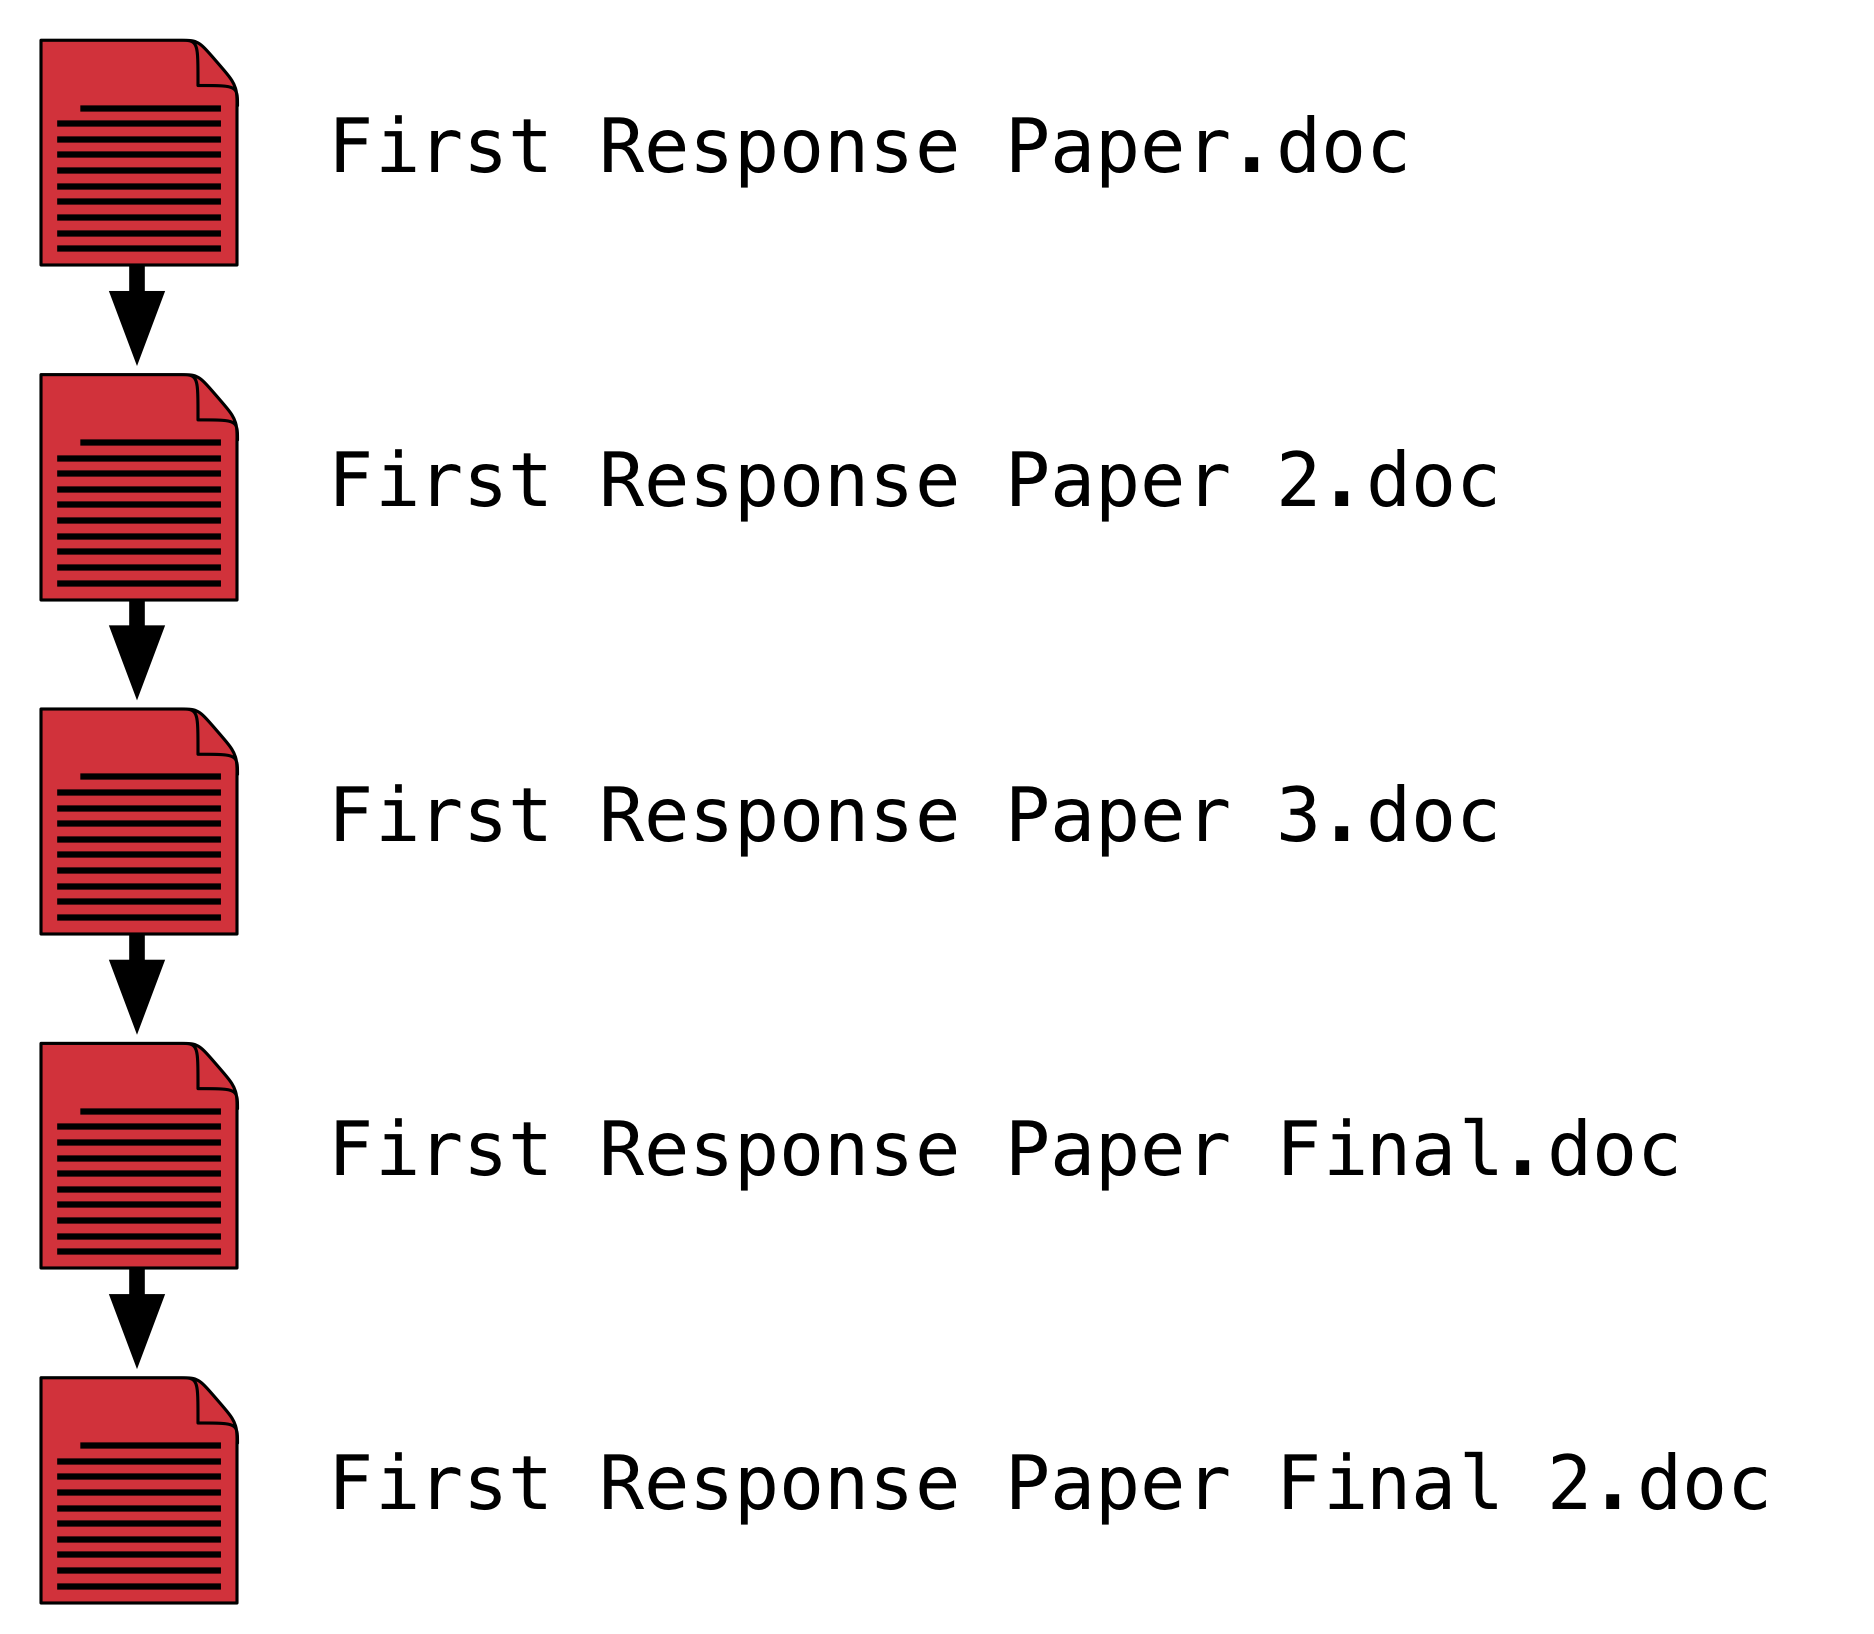
\includegraphics[width=0.5\linewidth]{images/gitFlow01}

The author made an initial copy of the paper, and then used a haphazard
and inconsistent approach for naming subsequent copies of the paper. We
can presume that changes were made in a linear fashion, though it is
easy to make changes to, say, \texttt{First\ Response\ Paper\ 2.doc}
after \texttt{First\ Response\ Paper\ 3.doc} has been created and
edited.

Instead of saving copies of their hypothetical paper, a student using
GitHub could write the paper in a single document, \textbf{commiting}
their changes as they progress to take ``snapshots'' of their progress.
These snapshots contain information on changes the student has made,
tracked line-by-line. So, at each point in which a new document would
have been created in the typical workflow, a student using GitHub would
simply \textbf{commit} their changes:

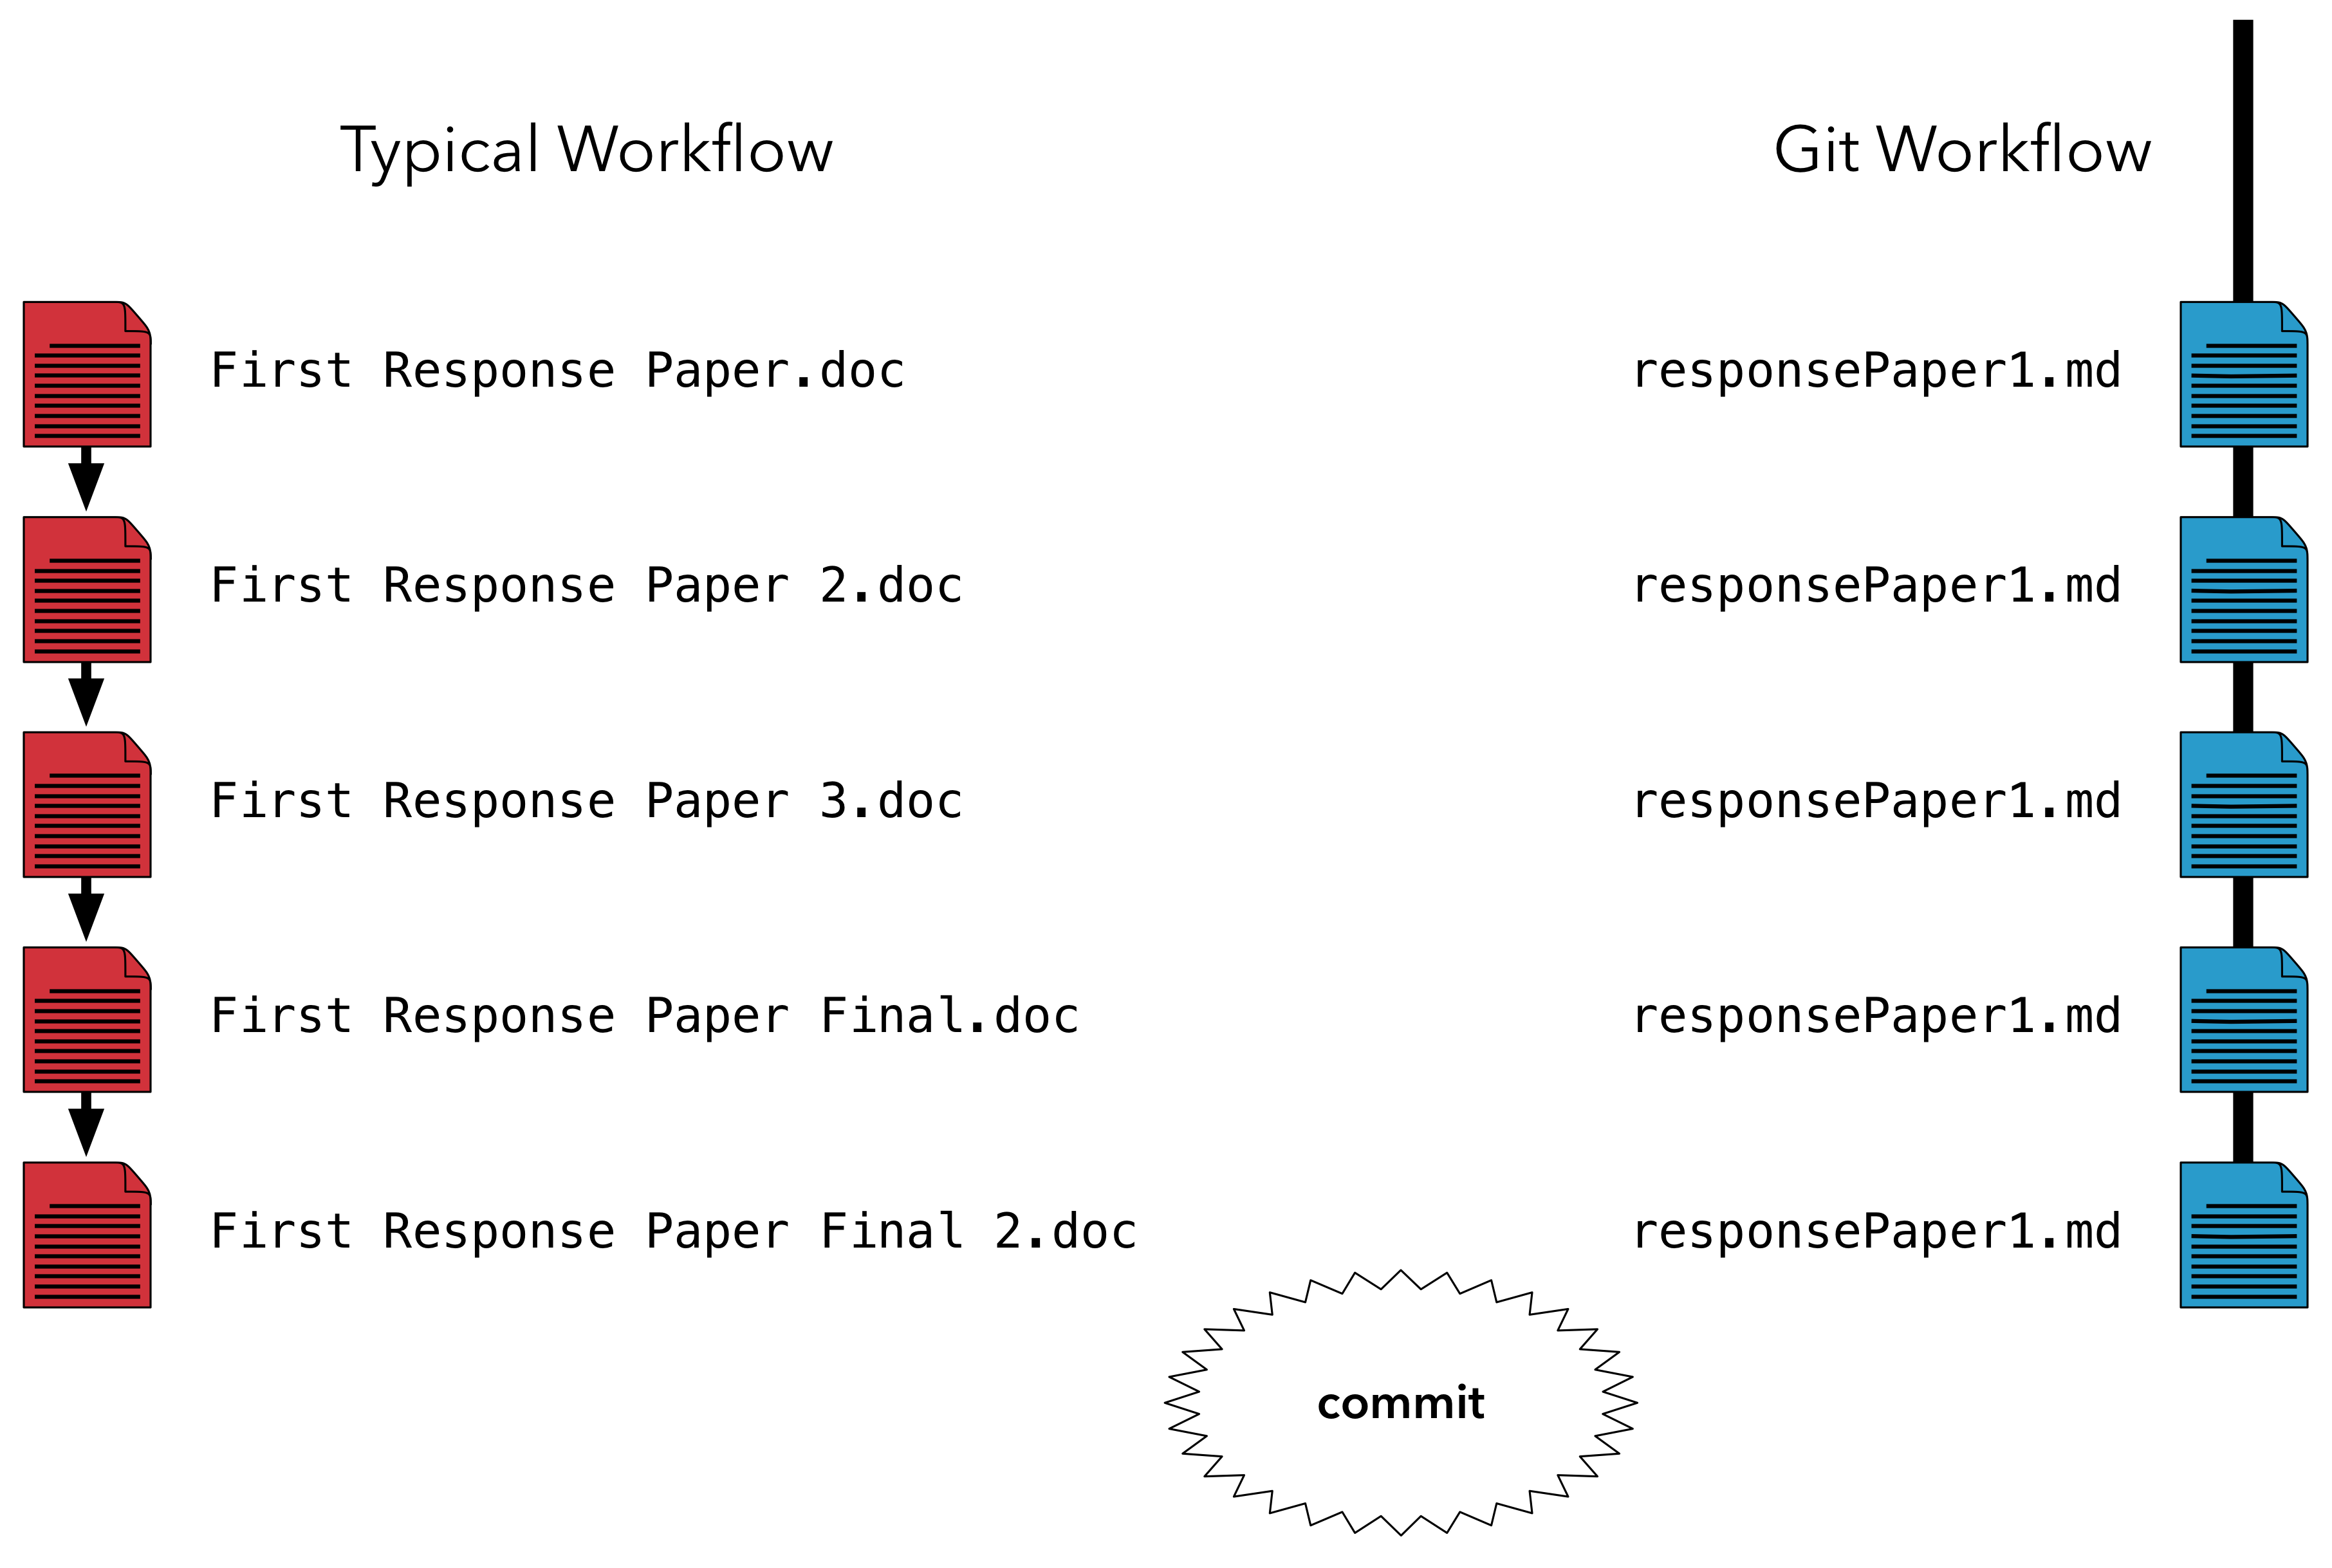
\includegraphics[width=1\linewidth]{images/gitFlow02}

Git provides a number of useful features beyond simply tracking changes.
Eachc commit is accompanied a \textbf{message}. These messages must have
a short summary that appears on GitHub and can also have a longer
description that can be used to describe in detail what changes are
being applied with a specific commit:

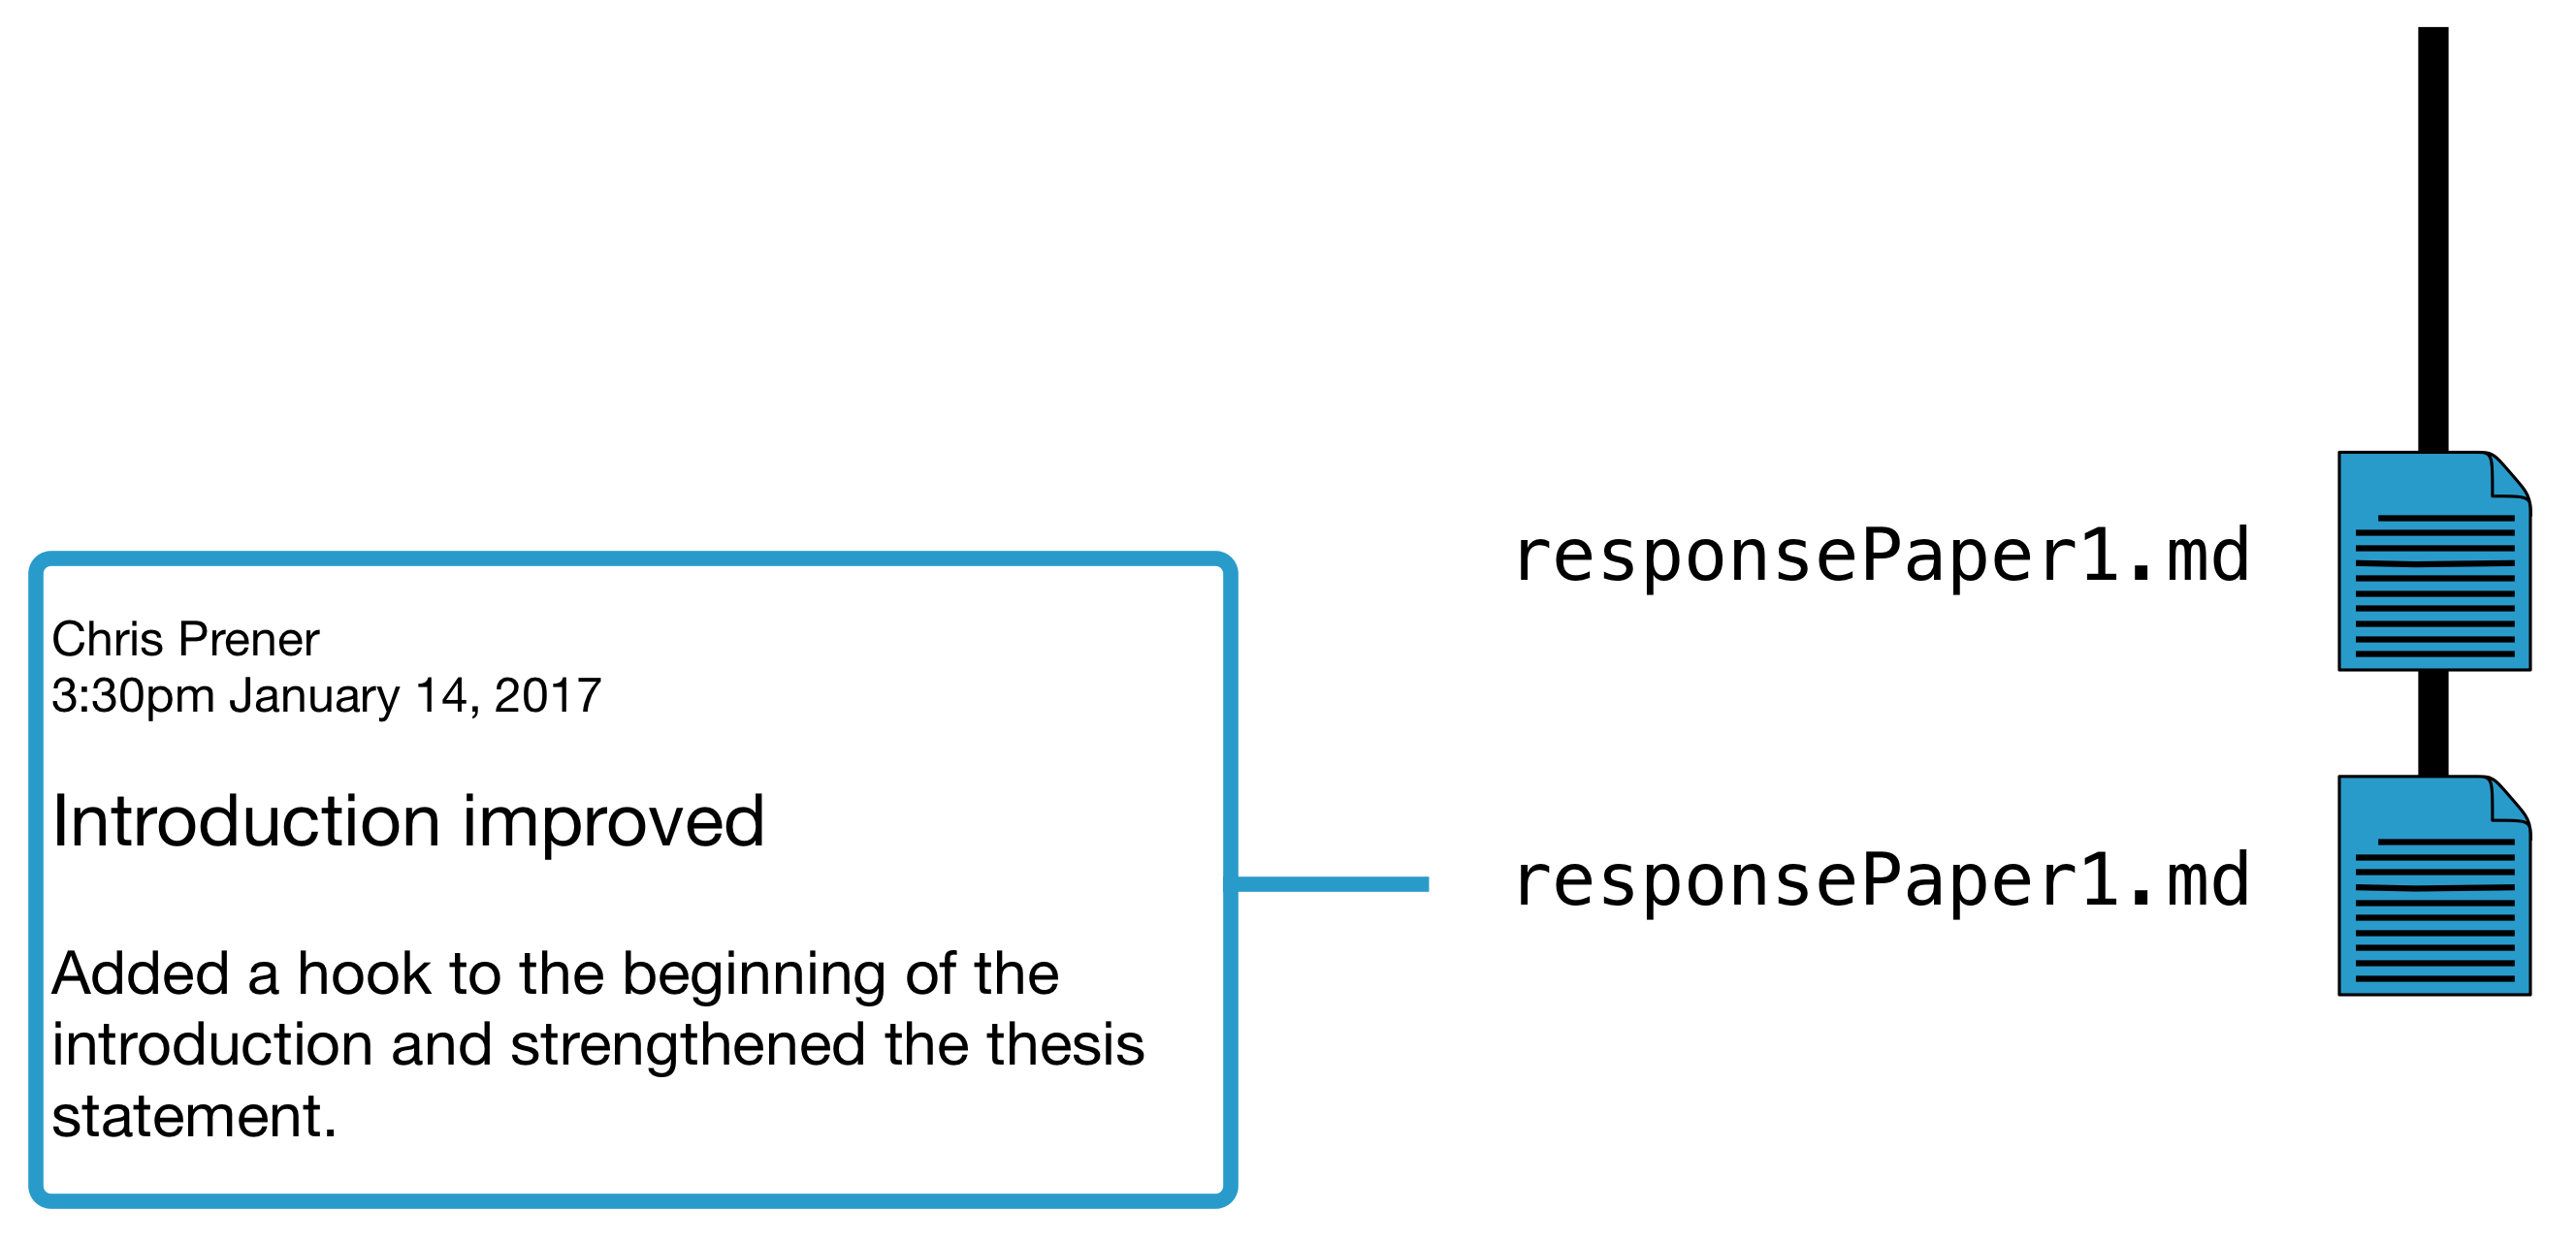
\includegraphics[width=1\linewidth]{images/gitFlow03}

Messages, combined with the changes that are tracked, allow users to
trace the development of a single document or an entire project
overtime:

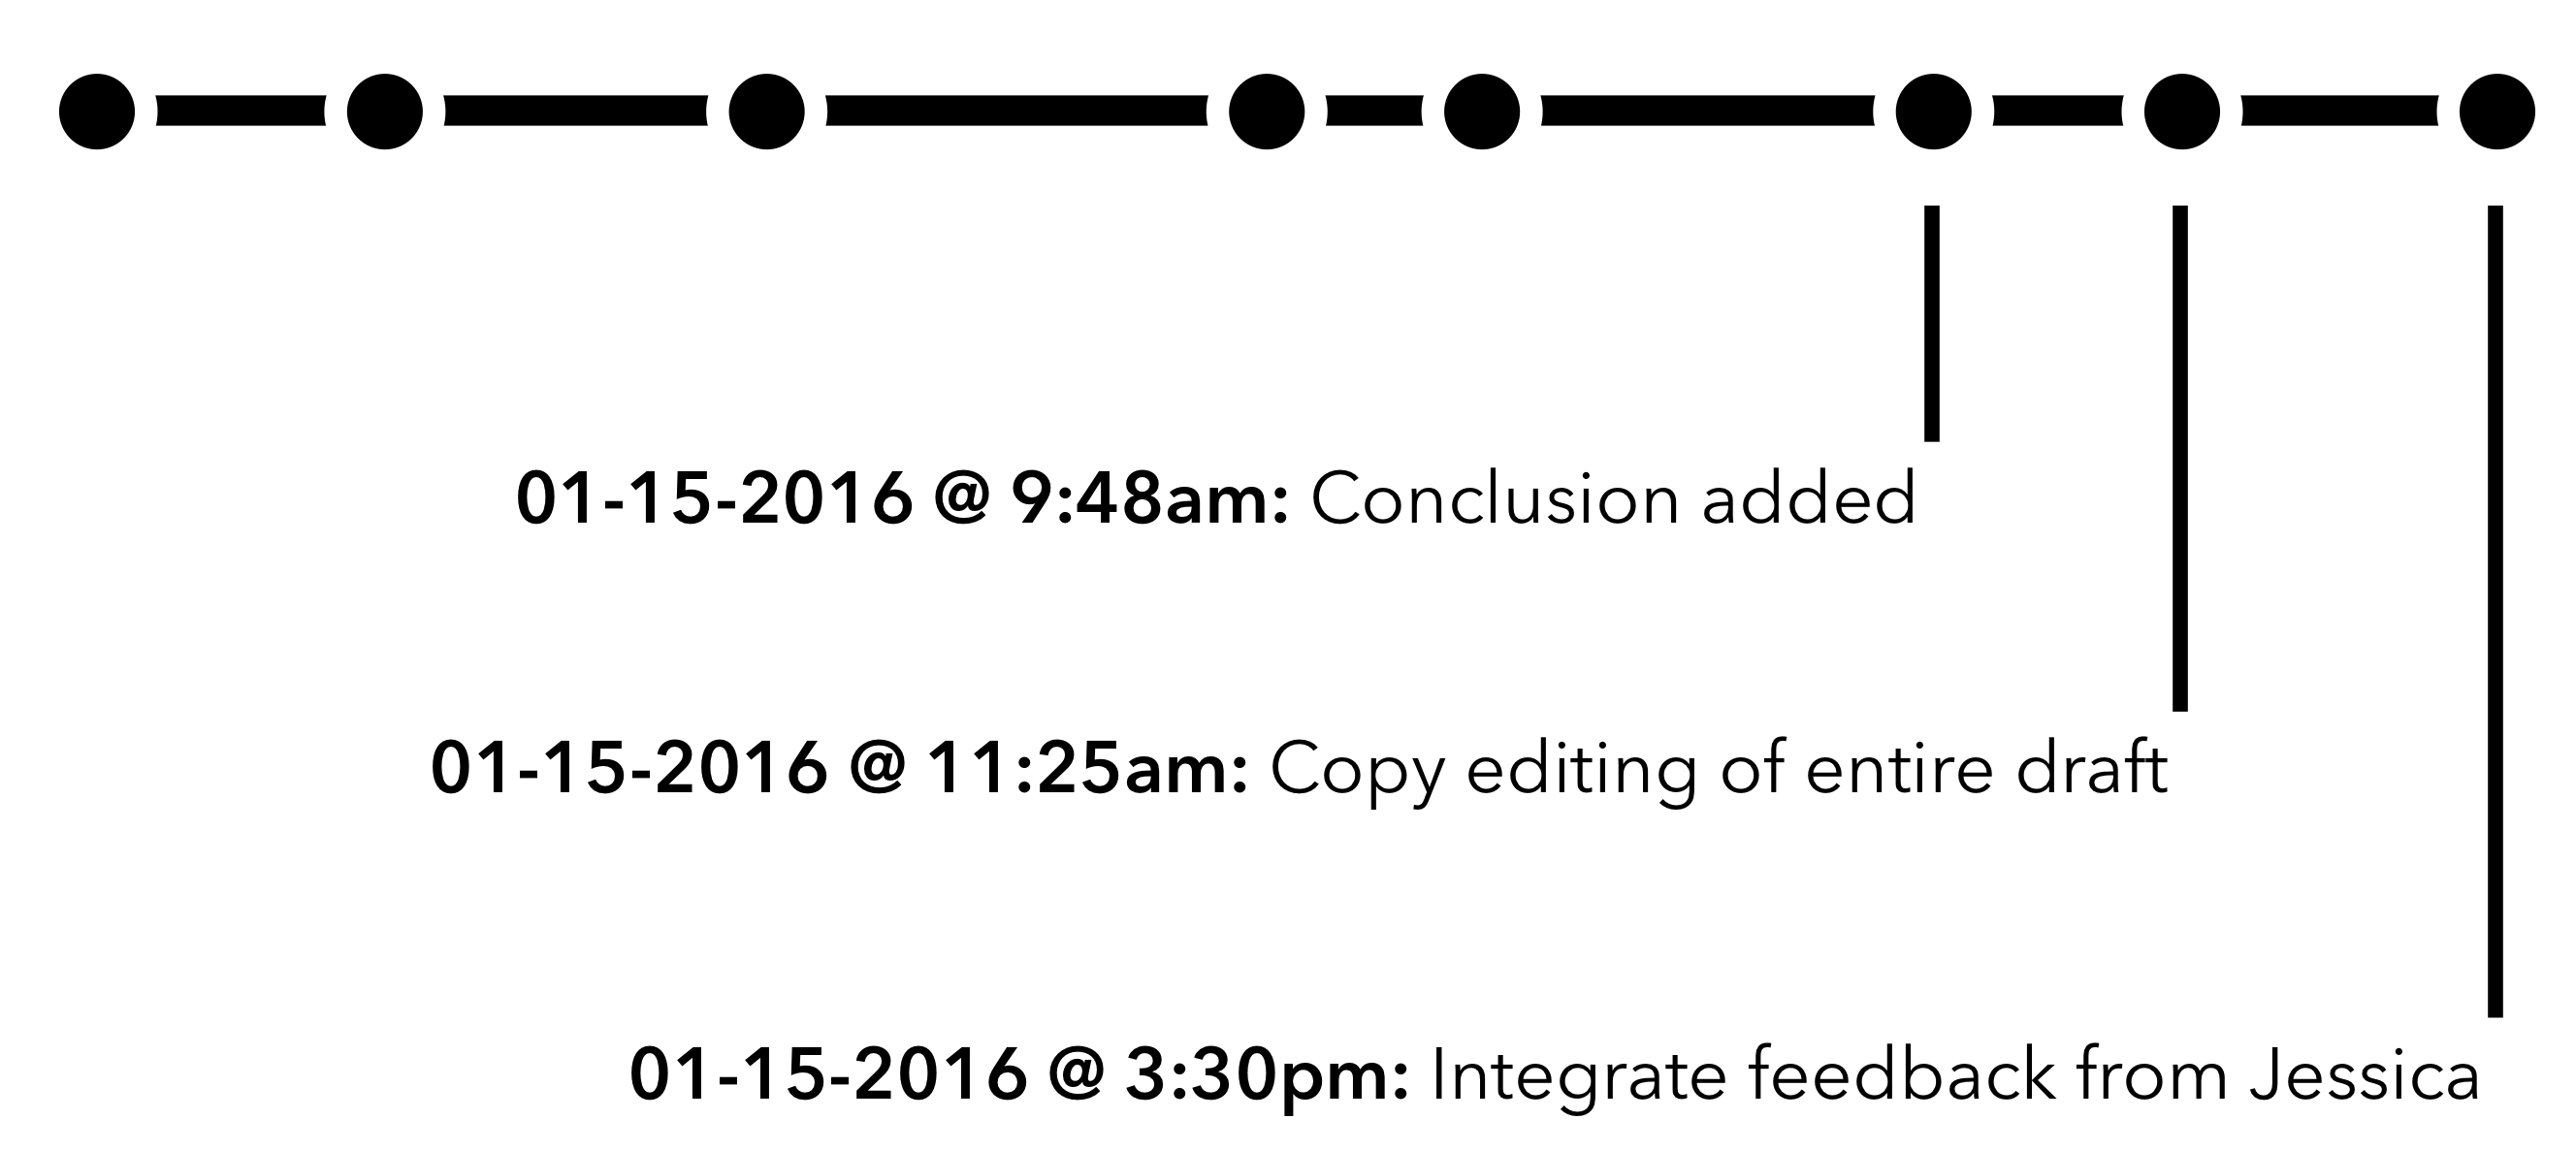
\includegraphics[width=1\linewidth]{images/gitFlow04}

This means that, if necessary, the project can also be rolled back to an
earlier period. Finally, users can \textbf{sync} their commits with
GitHub.com, hosting their changes and their data in a way that protects
them against certain types of computer failures and also allowing them
to easily share their work with others.

\section{GitHub Repositories}\label{github-repositories}

Users of GitHub.com adhere to a couple of norms with their repositories
that are worth knowing about. Repositories cannot have spaces in their
names (much like variables in Stata), so the naming conventions that we
will discuss in relation to Stata this semester all apply to GitHub as
well!

Public GitHub repositories also contain (typically) at least three core
files:

\begin{enumerate}
\def\labelenumi{\arabic{enumi}.}
\item
  A \textbf{license} file - since the data is out there for public
  consumption, it is important to think about how that data is licensed.
  The norm among GitHub users has been to use open source licenses,
  which let others edit and adapt your work. There are a range of
  \href{http://choosealicense.com}{licenses} that are commonly used on
  GitHub.
\item
  A \textbf{README} file - this describes the purpose and content of the
  project.
\item
  A \textbf{.gitignore} file - this stops certain types of files from
  being swept up by GitHub when a user syncs their files with a server.
\end{enumerate}

\section{Storing GitHub Repositories}\label{storing-github-repositories}

When you clone your repositories, you will be prompted to save them on
your computer. There are a number of ways in which this process can
introduce sources for trouble down the road. The principle way that I
have seen students run into problems with GitHub is by storing
repositories on cloud storage services like Dropbox or Google Drive. In
order to avoid any issues, I advise against storing GitHub repositories
in an area of your computer that syncs with a cloud service.

\section{GitHub Issues}\label{github-issues}

GitHub has a powerful tool for interaction called
\href{https://help.github.com/articles/about-issues/}{Issues}. These can
be accessed by opening a repository and then clicking on the ``Issues''
tab. Issues can be ``opened'' by anyone with access to the repository.
They allow for a conversation to occur in the form of messages posted
within the Issue itself. Files can be attached to Issues, and the
messages can contain Markdown formatting. Once the conversation is
complete, issues can be marked as ``closed'', which moves them into a
secondary view on the website so that they are archived.

We'll use issues for both assignment feedback and grading. Please keep
up with issues are they appear, and feel free to follow-up with specific
questions about your grade or the assignment feedback in the Issue
conversation. Once you are satisfied, please mark the issue as closed.

\section{GitHub Desktop Application}\label{github-desktop-application}

\href{https://desktop.github.com}{GitHub Desktop} is a tool that allows
you to easily clone repositories hosted on GitHub, commit changes to
them, and then sync those changes up to the website. You can also create
new repositories, however this is not task you will have to do this
semester. GitHub Desktop is not a fully functional desktop version of
GitHub. For our purposes, it is important to note that the Desktop
application will not let you easily identify when repositories have been
updated by other users, view Wikis associated with repositories, or view
Issues.

\section{Learning More}\label{learning-more}

GitHub has a
\href{https://help.github.com/articles/good-resources-for-learning-git-and-github/}{resources
page} with links to websites that are great for helping you learn more
about how Git and GitHub work! The next chapter also has some additional
GitHub and Git information.

One particularly great \href{https://try.github.io/}{tutorial} walks you
through the command line process for creating and using a git
repository. Even if you do not want to use Git via the command line, the
tutorial does an \emph{excellent} job of describing the logic and
sequence behind the Git workflow.

\bibliography{packages.bib,book.bib}


\end{document}
